%%%%%%%%%%%%%%%%%%%%%%%%%%%%%%%%%%%%%%%%%%%%%%%%%%%%%%%%%%%%%%%%%
% Qualificacao de Doutorado / Dept Fisica, CFM, UFSC            %
% Eduardo@UFSC - 2015                                           %
%%%%%%%%%%%%%%%%%%%%%%%%%%%%%%%%%%%%%%%%%%%%%%%%%%%%%%%%%%%%%%%%%

%:::::::::::::::::::::::::::::::::::::::::::::::::::::::::::::::%
%                                                               %
%                          Capítulo 2                           %
%                                                               %
%:::::::::::::::::::::::::::::::::::::::::::::::::::::::::::::::%

%***************************************************************%
%                                                               %
%                        EmLinesDataCube                        %
%                                                               %
%***************************************************************%

\chapter{Linhas de emissão}
\label{sec:emlines}

Os espectros observados carregam uma mistura de energia provenientes de diversas partes distintas
das galáxias (estrelas, gás, poeira, etc). Com a síntese de populações estelares pode-se modelar os
espectros de energias proveniente das estrelas de diferentes idades e composições químicas
(metalicidade), além da correção pela aplicação de alguma lei de extinção por poeira. Subtraindo os
espectros observados dos espectros modelados obtêm-se os espectros residuais, compostos pelas linhas
de emissão. Essas linhas são geradas principalmente através das ionizações e recombinações nos
níveis energéticos dos átomos dos elementos encontrados nas núvens de gás.

\section{EmLinesDataCube}
\label{sec:emline:datacube}

Nosso colaborador e membro do Projeto CALIFA {\em Survey}, Rubén García Benito, desenvolveu um
programa que, utilizando dos espectros residuais, faz a medida das linhas de emissão e erros
envolvidos no processo. Este programa faz parte do projeto e por enquanto não está aberto para
utilização da comunidade científica. Acreditamos que essas medidas sejam liberadas para a
comunidade científica assim que o último lançamento público de dados do CALIFA for feito (DR3).

Feitas as medidas dos fluxos integrados das linhas de emissão, temos o arcabouço para calcularmos
algumas propriedades que serão fundamentais em nossa pesquisa. Para isso escrevi um objeto em
\textsc{p}y\textsc{thon} que além de organizar os resultados das medidas dos fluxos das linhas de
emissão (provenientes do programa do Rubén) também calcula a abundância de oxigênio, um dos índices
usados como metalicidade nebular ($\log$ (O/H)), o coeficiente de extinção por decremento de Balmer
para as regiões nebublares ($\tauVN$), larguras equivalentes das linhas, assim como os erros
propagados em cada cálculo, etc. Esse objeto foi adicionado ao \pycasso
\citep{CidFernandes.etal.2013a} para que os demais membros do projeto possam utilizá-lo. Nesse
objeto encontram-se medidas do fluxo em diversas linhas de emissão, a posição central da linha,
amplitude, desvio padrão, equação para reconstrução do contínuo em cada linha de emissão, os erros
nestas medidas, além das propriedades mencionadas anteriormente e seus erros propagados.

\subsection{Extinção por decremento de Balmer}
\label{sec:emline:datacube:tauvneb}

Em um modelo que assume que entre o observador e a fonte de energia existe uma
camada difusa, como uma cortina, que extingue a luz diferentemente em cada comprimento de
onda, temos:
\begin{eqnarray}
   F_\lambda^{obs} &=& F_\lambda^{int} e^{-\tau_\lambda} \\
   F_\lambda^{obs} &=& F_\lambda^{int} e^{-(\frac{\tau_\lambda}{\tauV}) \tauV} \\
   \frac{\tau_\lambda}{\tauV} &=& q_\lambda \\
   F_\lambda^{obs} &=& F_\lambda^{int} e^{-q_\lambda \tauV} \\
   \frac{F_\lambda^{obs}}{F_{\lambda^\prime}^{obs}} &=& \
 \frac{F_\lambda^{int} e^{-q_\lambda \tauV}}{F_{\lambda^\prime}^{int} e^{-q_{\lambda^\prime} \tauV}} \\
   \ln \left(\frac{F_\lambda^{obs}}{F_{\lambda^\prime}^{obs}}\right) &=& \
 \tauV (q_{\lambda^\prime} - q_\lambda) \ln \left(\frac{F_\lambda^{int}}{F_{\lambda^\prime}^{int}}\right) \\
   \tauV &=& \frac{1}{(q_{\lambda^\prime} - q_\lambda)} \left[\ln \ 
 \left(\frac{F_\lambda^{obs}}{F_{\lambda^\prime}^{obs}}\right) - \
 \ln \left(\frac{F_\lambda^{int}}{F_{\lambda^\prime}^{int}}\right)\right] 
\end{eqnarray}

\noindent onde $F_\lambda$ é o fluxo em cada comprimento de onda, $\tau_\lambda$ é o coeficiente de
profundidade óptica para o comprimento de onda $\lambda$ e $\tauV$ é o coeficiente de profundidade
óptica na banda V.

A poeira existente ao redor das regiões de formação estelar é criada principalmente pela própria
formação estelar. Assumindo um modelo de extinção \citep[neste trabalho assumimos][]{CCM1989a},
podemos calcular qual o coeficiente de extinção para essas regiões nebulares. Para este cálculo
utilizamos o fato de que, apesar da extinção do espectro observado, a razão entre os fluxos
intrínsecos das linhas de \Halpha e de \Hbeta varia muito um pouco com a metalicidada, a densidade
e a temperatura. Usamos aqui esse valor como constante e igual a $2,86$
\citep{Osterbrock.Ferland.2006a}. Com isso temos:
\begin{equation}
	\tauVN = \frac{1}{(q_{\Hbeta} - q_{\Halpha})} \ln \left( \frac{F_{\Halpha}^{obs}/F_{\Hbeta}^{obs}}{2,86} \right).
\end{equation}
\noindent Nessa equação, os $q_\lambda$ são provenientes do modelo adotado. O erro propagado para
$\tauVN$ é:
\begin{eqnarray}
	\tauVN &\equiv& \tauVN(F_{\Halpha}^{obs}, F_{\Hbeta}^{obs}) \\
	\epsilon (\tauVN) &=& \sqrt{\left(\del{\tauVN}{F_{\Halpha}^{obs}}\right)^2 \
\epsilon (F_{\Halpha}^{obs})^2 + \left(\del{\tauVN}{F_{\Hbeta}^{obs}}\right)^2 \
\epsilon (F_{\Hbeta}^{obs})^2 } \\
	\del{\tauVN}{F_{\Halpha}^{obs}} &=& \frac{1}{F_{\Halpha}^{obs} (q_{\Hbeta} - q_{\Halpha})} \\
	\del{\tauVN}{F_{\Hbeta}^{obs}} &=& - \frac{1}{F_{\Hbeta}^{obs} (q_{\Hbeta} - q_{\Halpha})} \\
	\epsilon (\tauVN) &=& \frac{1}{(q_{\Hbeta} - q_{\Halpha})} \
\sqrt{\left(\frac{\epsilon (F_{\Halpha}^{obs})}{F_{\Halpha}^{obs}}\right)^2 + \
\left(\frac{\epsilon (F_{\Hbeta}^{obs})}{F_{\Hbeta}^{obs}}\right)^2 }
\end{eqnarray}

\subsection{Metalicidade Nebular}
\label{sec:emline:datacube:Zneb}

Os indicadores de metalicidade nebular (abundância de oxigênio no gás) mais utilizados são $\log$
(O3N2) e N2. As calibrações destes dois indicadores utilizadas pelo nosso projeto foram feitas por
\citet{Marino.etal.2013a} de forma empírica utilizando medidas de temperatura eletrônica de 603
regiões \Hii e mais medidas nebulares de 3423 regiões \Hii mapeadas por \citet{Sanchez.etal.2013a}.
O valor encontrado pelos autores foi:
\begin{equation}
	12 + \log \textrm{(O/H)} = 8.533[\pm0.012] - 0.214[\pm0.012]\times \textrm{O3N2}
\end{equation}
\noindent conforme pode ser vista na Fig. \ref{fig:Marino2013_O3N2}.

\begin{figure}
	\centering
	%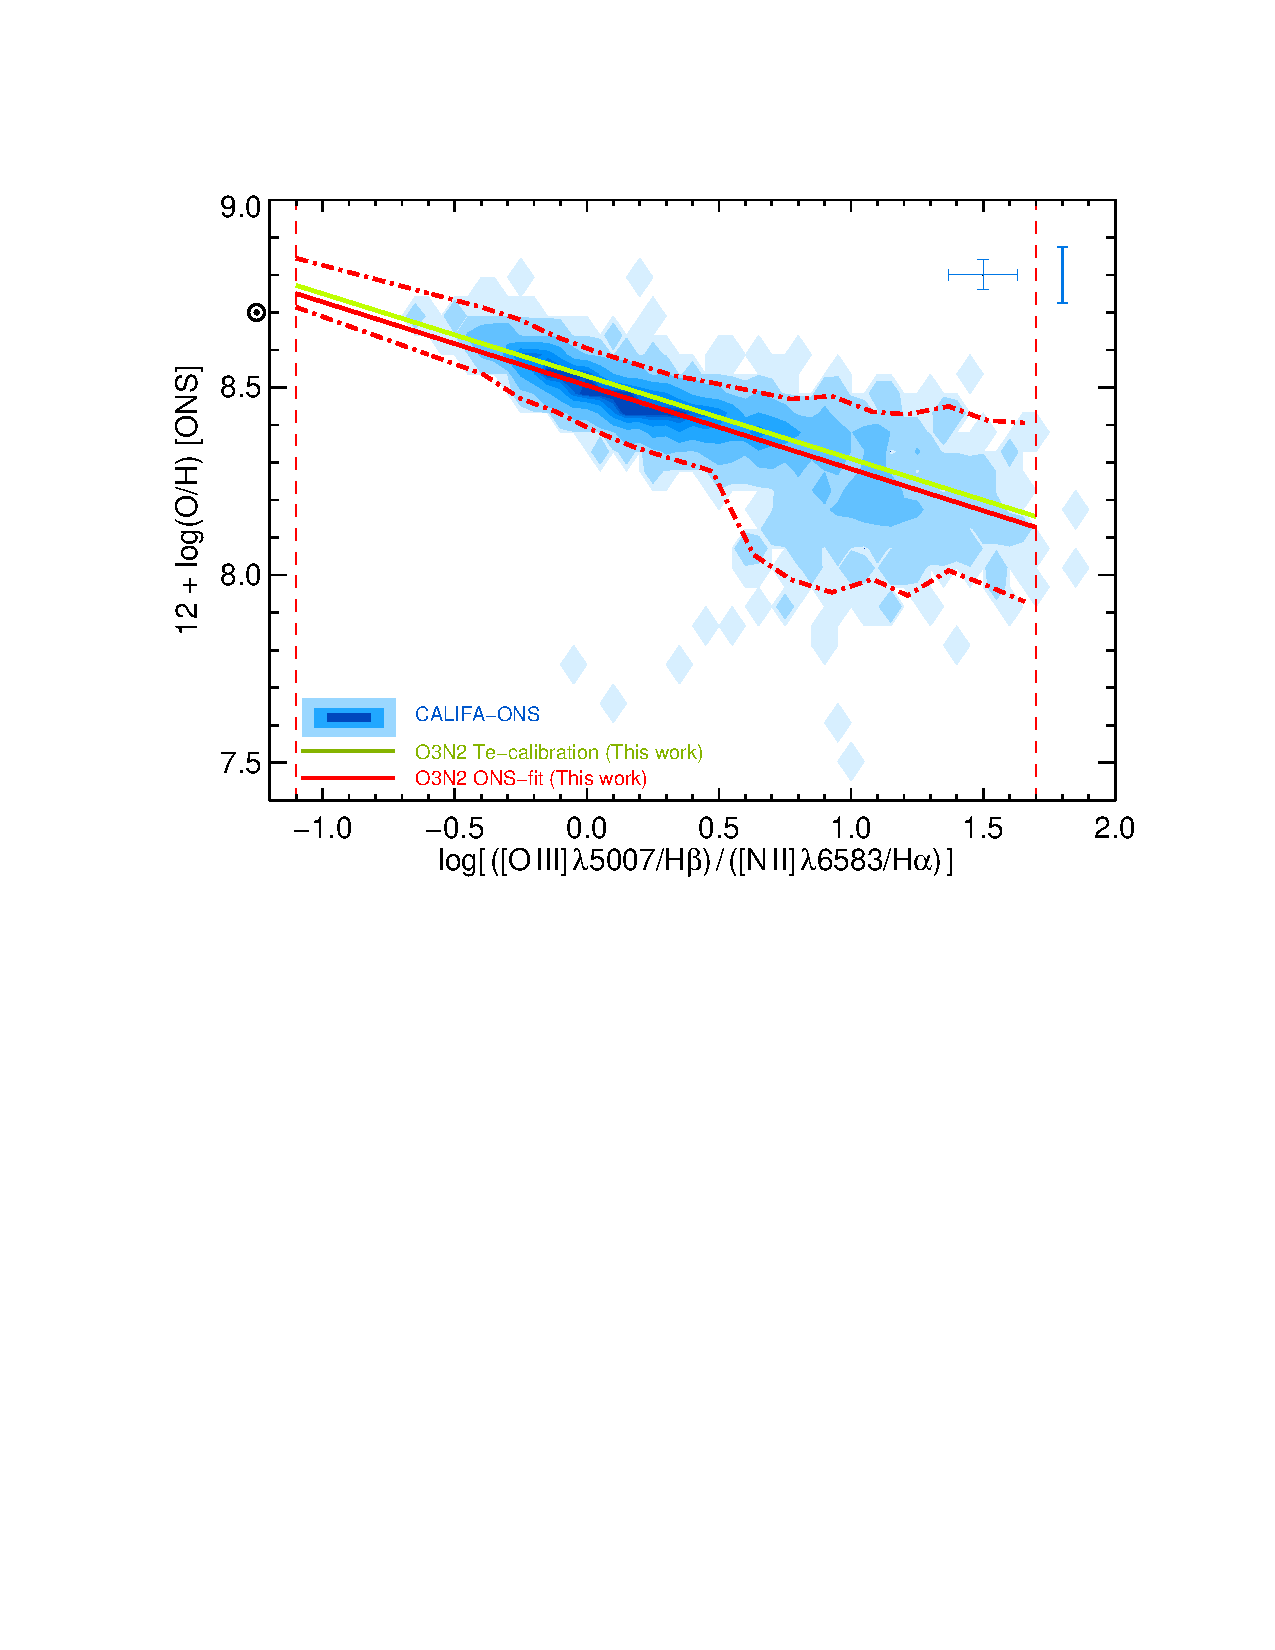
\includegraphics[width=0.3\columnwidth]{figuras/O3N2_CALIFA.pdf}
	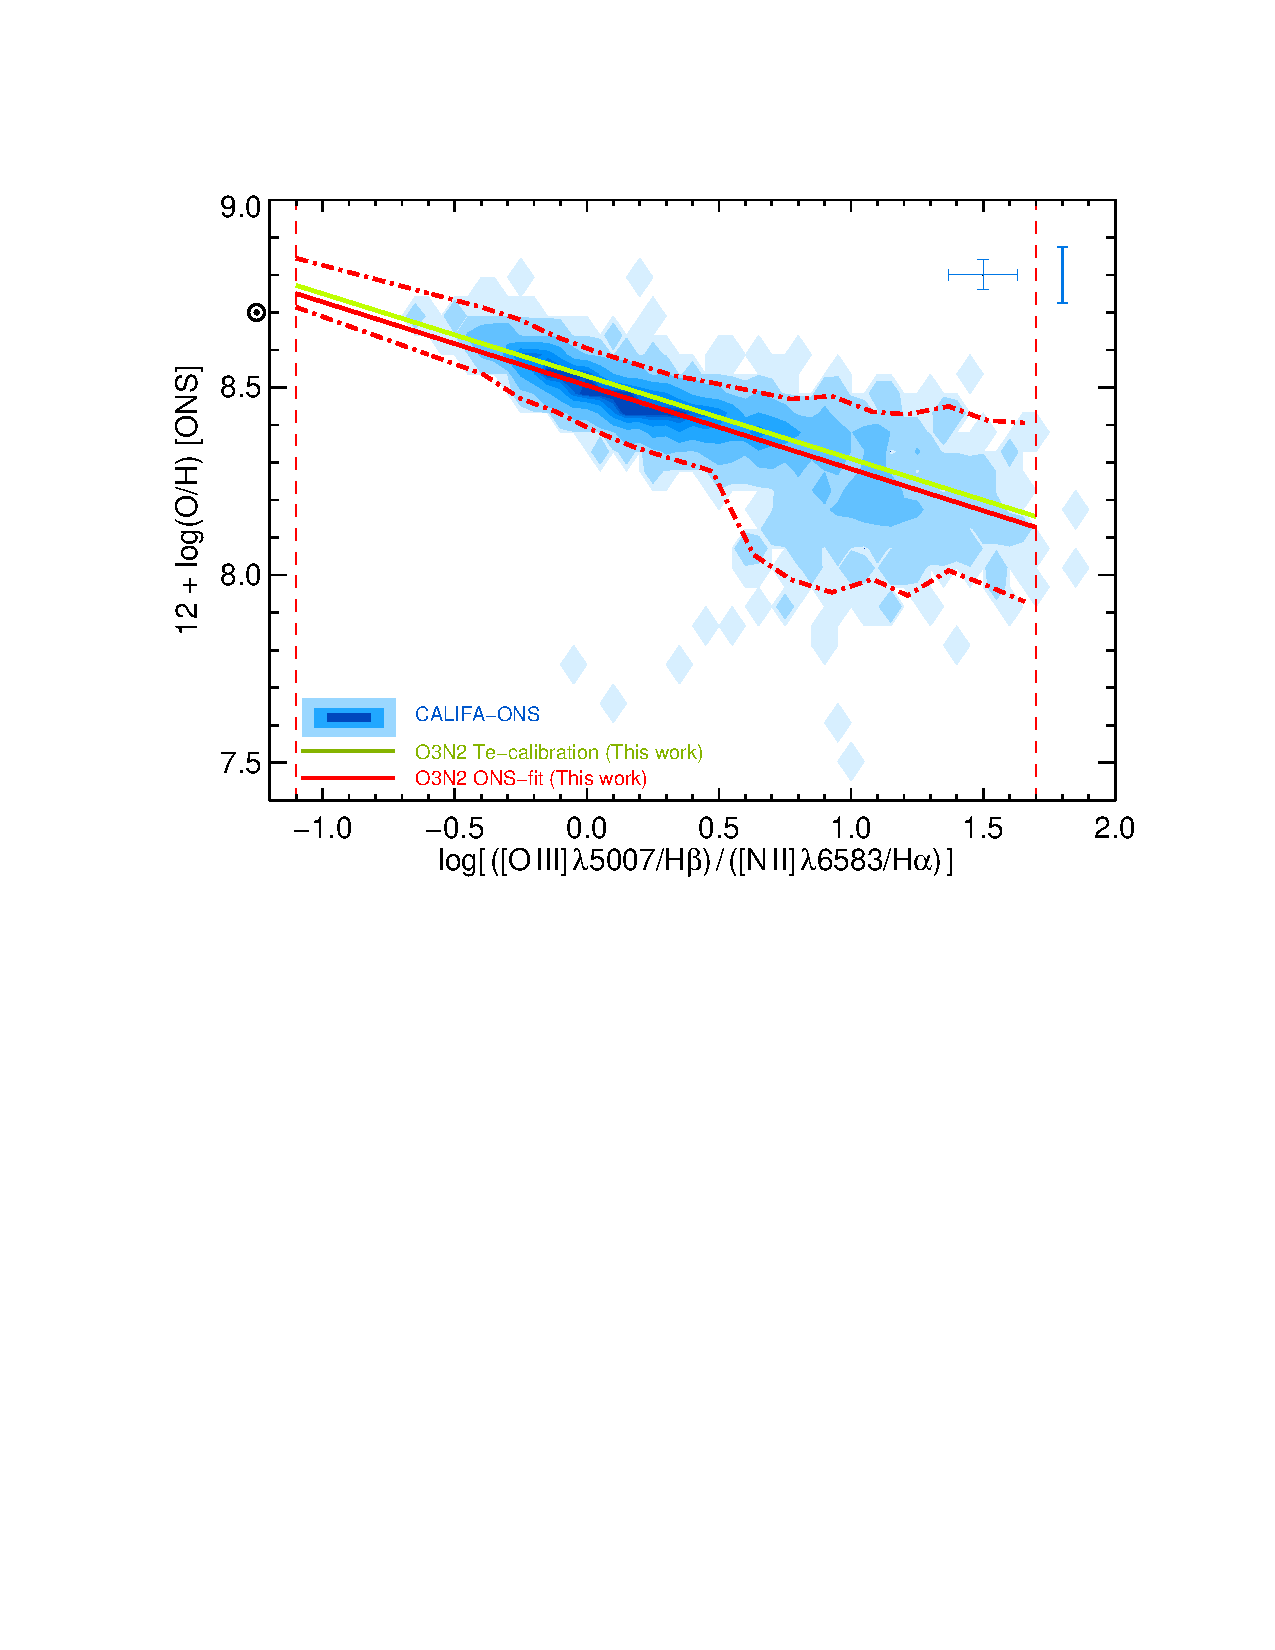
\includegraphics[scale=0.8, trim=2cm 13cm 2cm 3cm, clip]{figuras/O3N2_CALIFA.pdf}
	\caption[Calibração da abundância de oxigênio no gás]{Calibração da abundância de oxigênio 
	nebular	para 3423 regiões \Hii mapeadas por \citet{Sanchez.etal.2013a}. Figura retirada de 
	\citet{Marino.etal.2013a}}
	\label{fig:Marino2013_O3N2}
\end{figure}

\subsection{Exemplo de utilização}
\label{sec:emline:datacube:exemple}

Com a criação do objeto {\sc EmLinesDataCube} e adição ao \pycasso torna o processo de análise e
produção de gráficos extremamente simples. Podemos apreciar um exemplo de como produzir um gráfico
BPT \citep{Baldwin.Phillips.Terlevich.1981a} que utiliza fluxos de quatro linhas de emissão
(\Halpha, \Hbeta, \OIII e \NII) no código da Fig. \ref{fig:BPTprog} que resulta na Fig.
\ref{fig:BPTfig}.

\begin{figure}
	\begin{python}
import numpy as np
from matplotlib import pyplot as plt
from pycasso import fitsQ3DataCube

CALIFASuperFits='K0277.fits'
EmLinesFits='K0277.EML.fits'

# Carregando arquivos FITS
K = fitsQ3DataCube(CALIFASuperFits)
K.loadEmLinesDataCube(EmLinesFits)
# Agora todos as informacoes sobre as linhas de
# emissao estao instanciadas em K.EL

# Indices dos vetores aonde estao armazenados os
# fluxos de cada linha
i_Ha = K.EL.lines.index('6563')
i_Hb = K.EL.lines.index('4861')
i_O3 = K.EL.lines.index('5007')
i_N2 = K.EL.lines.index('6583')
Ha_obs__z = K.EL.flux[i_Ha, :]
Hb_obs__z = K.EL.flux[i_Hb, :]
N2_obs__z = K.EL.flux[i_N2, :]
O3_obs__z = K.EL.flux[i_O3, :]

# Razao entre os fluxos de N2/Ha e O3/Hb
N2Ha__z = np.log10(N2_obs__z) - np.log10(Ha_obs__z)
O3Hb__z = np.log10(O3_obs__z) - np.log10(Hb_obs__z)

# Grafico
f = plt.figure()
ax = f.gca()
sc = ax.scatter(N2Ha__z, O3Hb__z, c = K.zoneDistance_HLR,
           cmap = 'viridis', vmax = 2, vmin = 0,
           marker = 'o', s = 10, alpha = 0.8, edgecolor = 'none')
ax.set_xlabel(r'$\log\ [NII]/H\alpha$')
ax.set_ylabel(r'$\log\ [OIII]/H\beta$')
cb = plt.colorbar(sc)
cb.set_label('Radius [HLR]')
plt.axis([-1, 0.5, -1.5, 1])
f.savefig('%s-BPT.pdf' % K.califaID)
	\end{python}
	\caption[Exemplo de programa utilizando o EmLinesDataCube.]
	{Exemplo de programa utilizando os fluxos de \Halpha, \Hbeta, \OIII e \NII 
	para construção de um gráfico BPT.}
	\label{fig:BPTprog}
\end{figure}

\begin{figure}
	%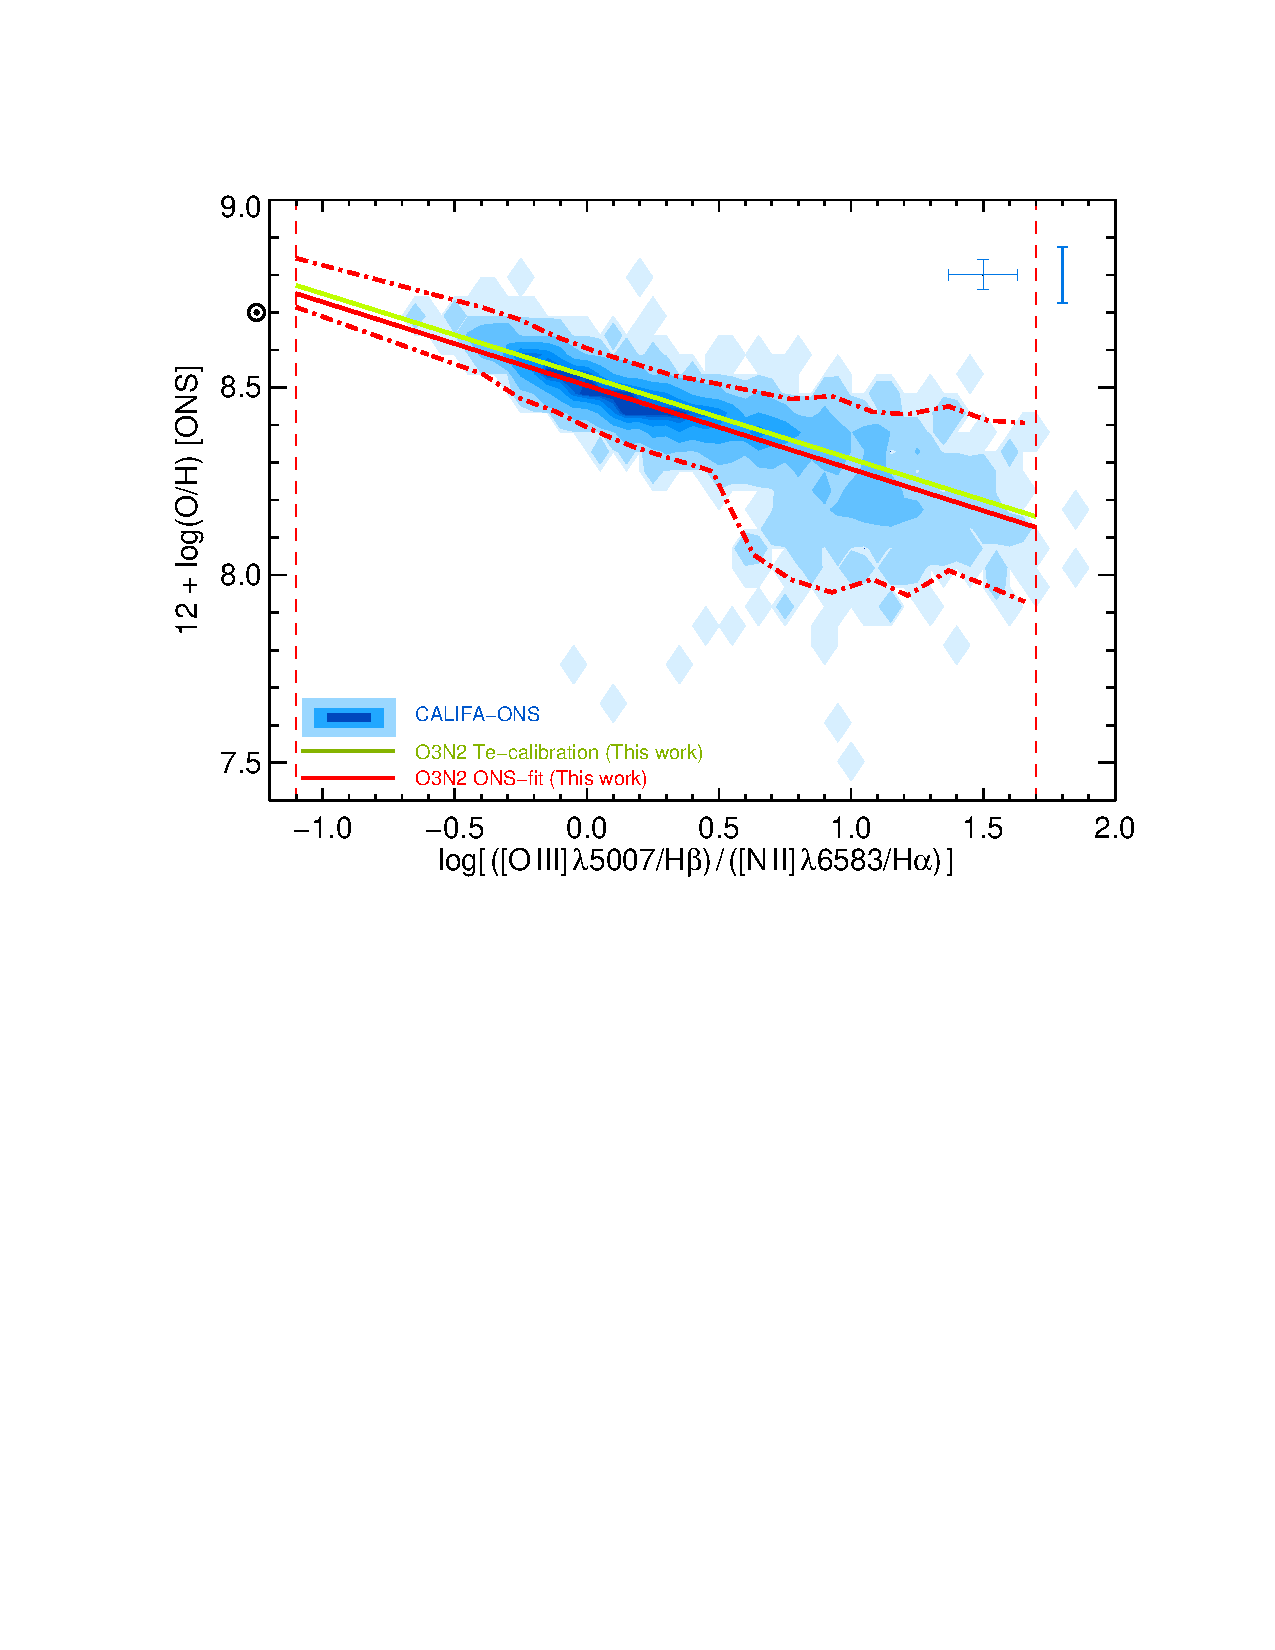
\includegraphics[scale=0.8, trim=2cm 13cm 2cm 3cm, clip]{figuras/O3N2_CALIFA.pdf}
	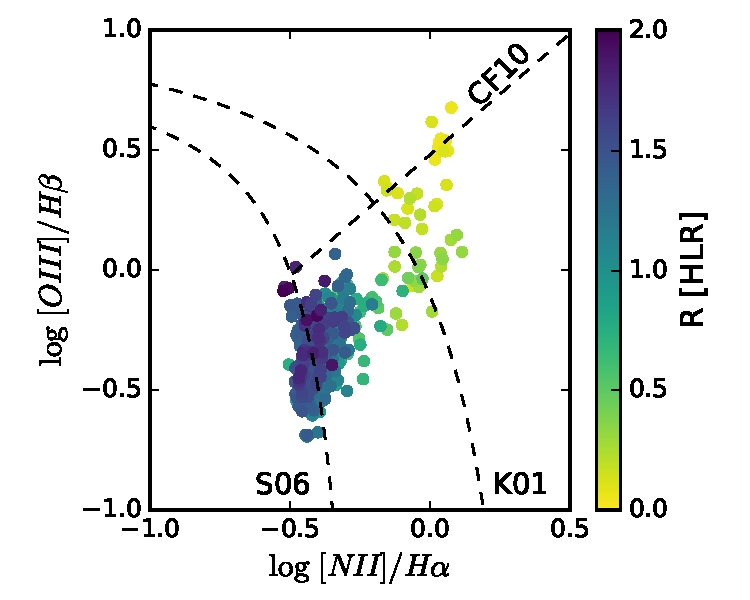
\includegraphics[scale=0.85]{figuras/K0277-BPT.pdf}
	\caption[Diagrama BPT produzido pelo programa de exemplo.]
	{Diagrama BPT produzida pelo exemplo \ref{fig:BPTprog}. Nela utiliza-se os fluxos de
	\Halpha, \Hbeta, \OIII e \NII.}
	\label{fig:BPTfig}
\end{figure}

\section{Taxa de formação estelar}
\label{sec:emlines:SFR}

Um dos métodos mais usados e difundidos para medida de taxa de formação estelar \footnote{Daqui por
diante usarei a sigla SFR - {\em Star Formation Rate}} recente utiliza a linha de emissão de
\Halpha. Nesse método assume-se que a formação estelar é constante nos últimos $t$ anos, a idade das
estrelas massivas ionizantes, que produzem basicamente todos os fótons que geram a linha de emissão
de \Halpha.

Nós queremos calibrar a luminosidade da linha de \Halpha ($\mathrm{L}_{\Halpha}$) como um indicador
de SFR ($\psi$) \citep[e.g., ][]{Kennicutt.1998a} usando uma relação linear:
\begin{equation}
	\psi_{\Halpha} = k \times \mathrm{L}_{\Halpha}.
	\label{eq:SFRHa}
\end{equation}
\noindent Portanto, nosso trabalho é encontrar $k$.

A quantidade total de luz $l$\footnote{$l(t)$ pode ser qualquer função que descreve a evolução
temporal de qualquer fonte raditiva genérica \emph{por unidade de massa formada} (portanto,
dependente da {\em Initial Mass Function - IMF}) de uma população estelar simples ({\em Simple
Stellar Population} - SSP)} que recebmos de estrelas que se formaram $t$ anos atrás é:
\begin{equation}
	\mathrm{d}\Lambda = l(t)\ \mathrm{d}\mathrm{M}(t).
	\label{eq:dLambda}
\end{equation}
\noindent No entanto, para obter $\Lambda$ nós temos que saber como a massa em estrelas cresce no
tempo (SFR) e isso não é possível diretamente por esse método. Integrando a equação
\eqref{eq:dLambda} dentro do tempo do Universo $T_U\ \sim$ 14Gyr), nós teremos hoje, um total de 
\begin{eqnarray}
	\mathrm{d}\mathrm{M}(t) &=& \psi(t)\ \mathrm{d}t \\
	\Lambda = \Lambda(t = T_U) &=& \int_0^{T_U} l(t)\ \textrm{d}\textrm{M}(t) = \int_0^{T_U} \psi(t)\
	l(t)\ \textrm{d}t
	\label{eq:Lambda}
\end{eqnarray}
\noindent luz $l$. Assumindo o caso B de recombinação do hidrogênio, um em cada 2.226 fótons
ionizantes produzem um fóton de \Halpha. Esse número não varia muito em função da temperatura e da
densidade nas regiões nebulares. Por fim a luminosidade intrísica de \Halpha pode ser teoricamente
calculada como:
\begin{equation}
	\mathrm{L}(\Halpha) = h \nu_{\Halpha} \frac{\mathrm{Q}_H}{2.226},
	\label{eq:LHa_recomb_theory}
\end{equation}
\noindent aonde $\mathrm{Q}_H$ é a taxa de fótons H-ionizantes. Em todo este processo
assume-se que nenhuma radiação escapa da núvem e, apesar de $\mathrm{L}(\Halpha)$ estar corrigido
por extinção, também assume-se que a poeira não espalha muito os fótons com $h\nu\ < 13.6 eV$.
Escrevemos $dQ_H$ como a equação \eqref{eq:dLambda}. Integrando como a equação \eqref{eq:Lambda}
obtemos:
\begin{eqnarray}
	Q_H &=& \int dQ_H = \int q_H(t)\ \mathrm{d}\mathrm{M}(t) \\ 
	Q_H(t = T) &=& \int_0^T \psi(t)\ q_H(t)\ dt
	\label{eq:QH}
\end{eqnarray}
\noindent Nas equações acima, $q_H$ é a taxa de fótons H-ionizantes por unidade de massa formada.
Nós podemos utilizá-lo como nosso tipo de luz $l$ na equação \eqref{eq:Lambda} considerando os
fótons que possam ionizar o hidrogênio (h$\nu\ \geq\ 13.6$ eV ou $\lambda\ \leq\ 912\AA$) e assim
escrever:
\begin{equation}
	q_H(t) = \int_0^{912\AA} \frac{l_\lambda\ \lambda}{h c} d\lambda.
	\label{eq:qH}
\end{equation}
\noindent Nesta equação, $l_\lambda$ é a luminosidade por unidade de massa formada e comprimento de
onda em unidades solares $[\textrm{L}_\odot/\AA\textrm{M}_\odot]$ para uma SSP\footnote{Apesar de
não escritas aqui, existem dependências com Z, função inicial de massa ({\em Initial Mass Function}
- IMF) e isócronas em $l_\lambda$ (portanto, também em $q_H$ e todos os seus produtos)}. Com isso,
nós ainda precisamos analisar como a integração de $q_H$ evolui com o tempo, para então obter
a SFR ($\psi$). Integrando $q_H$ de hoje até $T_U$ nós obtemos o número de fótons H-ionizantes
produzidos pelas fontes que emitem a luz $l$:
\begin{equation}
	\mathcal{N}_H = \int_0^{T_U} q_H(t)\ dt
\end{equation}
Para nossa configuração de modelos podemos ver a evolução de $\mathcal{N}_H$ no tempo na Fig.
\ref{fig:Nh_qh}. Esta figura mostra a evolução de $\mathcal{N}_H$ no tempo, em valores absolutos
(painel superior esquerdo) e relativamente ao total de $\mathcal{N}_H$ (painel superior direito).
Em \citet[Fig. 2b]{CidFernandes.etal.2011a} nós podemos ver a evolução temporal de $q_H$ sob
todas as idades e metalicidades\footnote{Naquele estudo, o grupo
\href{http://starlight.ufsc.br}{SEAGal/\STARLIGHT} usou as isócronas de Padova 1994 com a IMF de
\citet{Chabrier.2003a}}. A mesma figura é reproduzida no painel inferior. É notável que o número de
fótons H-ionizantes rapidamente converge ao máximo perto de $t = 10$ Myr. Para uma SFR constante
dentro dessa escala temporal ($\psi(t)\rightarrow \psi$) a equação \eqref{eq:QH} converge
para
\begin{equation}
	Q_H = \psi\ \mathcal{N}_H(t\ =\ 10\ \textrm{Myr, IMF, Z}{}_\star).
	\label{eq:QH_converge}
\end{equation}
\noindent Substituindo \eqref{eq:QH_converge} em \eqref{eq:LHa_recomb_theory} podemos escrever:
\begin{equation}
	\psi_{\Halpha} = \frac{2.226}{\mathcal{N}_H\ h \nu_{\Halpha}} \times \mathrm{L}(\Halpha)
	\label{eq:SFR_theoric}
\end{equation}
\noindent Este método nos dá uma SFR recente, em termos de que usamos o valor de $N_H$ para $t = 10$
Myr. Finalmente, resolvendo \eqref{eq:SFR_theoric} encontramos o valor para $k$ em \eqref{eq:SFRHa}
($\psi \equiv \mathrm{SFR}$):
\begin{equation}
	\label{eq:SFRNeb}
	\mathrm{SFR}_{\Halpha} = 3.13\ \mathrm{M}_\odot\ yr^{-1}
	\left(\frac{\mathrm{L}(\Halpha)}{10^8\mathrm{L}_\odot}\right)
\end{equation}

\begin{figure}
	%\resizebox{0.99\textwidth}{!}{\includegraphics{Nh_logt_metBase_Padova2000_salp.pdf}}
	\includegraphics[scale=0.62]{figuras/Nh_logt_metBase_Padova2000_salp.pdf}
	\caption{\emph{Painel superior esquerdo}: A evolução no tempo do número de fótons ($\mathcal{N}_H$)
para 6 metalicidades (de 0.02 $Z_\odot$ até 1.58 $Z_\odot$) que compoem nossos modelos de SSP.
A linha preta grossa representa a evolução utilizando metalicidade solar. \emph{Painel superior
direito}: O mesmo que o \emph{painel superior esquerdo} mas normalizado pelo valor total de
$\mathcal{N}_H$. A linha pontilhada representa 95\% do total de $\mathcal{N}_H$.
Em destaque a região ao redor de 10 Myr. \emph{Painel inferior}: Evolução da taxa de fótons
H-ionizantes em unidades da massa formada. Também mostra o valor seguindo o código de cores para as
mesmas metalicidades.}
	\label{fig:Nh_qh}
\end{figure}
 
% End of this chapter
